\documentclass[11pt,a4paper]{article}
\author{TalentSprint}
\date{}
\usepackage{verbatim}
\usepackage{fancyhdr}           % For header and footer
\usepackage{multicol}
\usepackage{colortbl}           % For coloured tables
\usepackage{setspace}           % For line height
\usepackage{seqsplit}           % Splits long words.
\usepackage{amsmath} 
\usepackage{graphicx}
\usepackage{array}
\usepackage{enumitem}
\usepackage{xcolor}
\usepackage[tikz]{bclogo}
\usepackage{textcomp}
\usepackage{listings}
\lstset{language=python,numbers=left,numberstyle=\tiny,numbersep=10pt,showstringspaces=false}

\headheight=14pt
\lhead{\nouppercase{}}
\rhead{\nouppercase{\leftmark}}

\newcommand*\lstinputpath[1]{\lstset{inputpath=#1}}
\lstinputpath{../Code/}
\graphicspath{{../Images/} {../ScreenShots/}}

\setcounter{tocdepth}{1}
\setlength\parindent{0pt}
\parskip=4pt
\newcommand{\Code}[1]{\textbf{\texttt{#1}}}

% Lengths and widths
\addtolength{\textwidth}{5cm}
\addtolength{\hoffset}{-1cm}
\setlength{\headsep}{-12pt} % Reduce space between header and content
\setlength{\headheight}{85pt} % If less, LaTeX automatically increases it
\renewcommand{\footrulewidth}{2pt} % Remove footer line
\renewcommand{\headrulewidth}{1pt} % Remove header line
\renewcommand{\seqinsert}{\ifmmode\allowbreak\else\-\fi} % Hyphens in seqsplit
% This two commands together give roughly
% the right line height in the tables
\renewcommand{\arraystretch}{1.3}
\onehalfspacing

% Commands
\newcommand{\SetRowColor}[1]{\noalign{\gdef\RowColorName{#1}}\rowcolor{\RowColorName}} % Shortcut for row colour
\newcommand{\mymulticolumn}[3]{\multicolumn{#1}{>{\columncolor{white}}#2}{#3}} % For coloured multi-cols
\newcolumntype{x}[1]{>{\raggedright}p{#1}} % New column types for ragged-right paragraph columns
\newcommand{\tn}{\tabularnewline} % Required as custom column type in use

% Font and Colours
\definecolor{HeadBackground}{HTML}{333333}
\definecolor{FootBackground}{HTML}{666666}
\definecolor{TextColor}{HTML}{333333}
\definecolor{DarkBackground}{HTML}{6B8E23} %{FD1AA8}
\definecolor{LightBackground}{HTML}{E8FED8} %D3FDC8
\definecolor{tit}{HTML}{FF6600}
\renewcommand{\familydefault}{\sfdefault}
\color{TextColor}
 \headsep = 25pt
% Header and Footer
\pagestyle{fancy}
\usepackage[headheight=110pt]{geometry}
\fancyhf{}% Clear header/footer

\fancyhead[r]{
\includegraphics[width = 4cm, height = 2cm]{TS-Logo.png}\hspace{0cm}}

%=================================TITLE=====================================
\fancyhead[l]{\Large{\bf{\textcolor{tit}{\textrm{File Handling}}}}}
%===========================================================================

\renewcommand{\headrulewidth}{0.4pt}% Default \headrulewidth is 0.4pt
\renewcommand{\footrulewidth}{0.4pt}% Default \footrulewidth is 0pt

\rfoot{Page \thepage}
\lfoot{COPYRIGHT \textcopyright TALENTSPRINT, 2015. ALL RIGHTS RESERVED.}

\begin{document}


%\chapter{File Handling}
\section*{Introduction}
File is a place on disk where a group of related data is stored. For example we can store characters, words, lines, paragraphs and pages from a textual document, fields and records belonging to a database; or pixels from a graphical image in a file.

In order to store information permanently and retrieve it  we need to use files. A file represents a sequence of bytes, does not matter if it is a text file or binary file. C language provides access on high level functions as well as low level (OS level) calls to handle file on your storage devices.

Why files are needed? When the program is terminated, the entire data is lost. If you want persist some data across different runs of a program (like the highest score in a game) you need to permanently store that information. That is where files come in. 

Files can be categorized as: 
\begin{itemize}
  \item text files and 
  \item binary files.
\end{itemize}

Text files are human readable, while binary files are not. We will only see how to handle text files in these notes.

\section*{Working with files}
FILE pointer is \texttt{struct} defined in standard library.

File pointer is capable of managing all the information needed to handle a stream, including its file position indicator, a pointer to the associated buffer (if any), an error indicator that records whether a read/write error has occurred, and an end-of-file indicator that records whether the end of the file has been reached. The declaration is: 

\lstinline!FILE* fp;! 

\subsection*{Opening a file} 
The \texttt{fopen()} function is used to create a new file or to open an existing file. This call will initialize an object of the type FILE. Following is the prototype of this function call:

 \lstinline!FILE* fopen(const char* filename, const char* mode);!

Here, filename is string literal, which you will use to name your file and access mode can have one of the following values:

\begin{table}[ht]
\begin{center}
\begin{tabular}{|c|c|}\hline
\textbf{Mode} & \textbf{Description}\\ \hline
r  & Opens an existing text file for reading purpose.\\ \hline
w  & Opens a text file for writing, if it does not exist then a new file is created.\\
   & Here your program will start writing content from the beginning of the file.\\ \hline
a  & Opens a text file for writing in appending mode, \\
   & if it does not exist then a new file is created. \\
   & Here your program will start appending content in the existing file content.\\ \hline
r+ & Opens a text file for reading and writing both.\\ \hline
w+ & Opens a text file for reading and writing both. \\
   & It first truncate the file to zero length if it exists otherwise\\
   & create the file if it does not exist.\\ \hline
a+ & Opens a text file for reading and writing both.\\
   & It creates the file if it does not exist. The reading will start \\
   & from the beginning but writing can only be appended.\\ \hline
\end{tabular}
\end{center}
\end{table}
If you are going to handle binary files then you will use below mentioned access modes instead of the above mentioned: 

``rb'', ``wb'', ``ab'', ``rb+'', ``r+b'', ``wb+'', ``w+b'', ``ab+'', ``a+b''.

If the \texttt{fopen()} call is successful a valid FILE handle is returned. If the call failed, NULL is returned.

\subsection*{Closing a File}
After finishing the reading or writing to a file, it must be closed. Otherwise you run the risk of losing the data and/or corrupting the contents of the file.

To close a file, use the \texttt{fclose()} function. The prototype of this function is: \lstinline!int fclose( FILE* fp );! The \texttt{fclose()} function returns zero on success, or EOF if there is an error in closing the file. This function actually, flushes any data still pending in the buffer to the file, closes the file, and releases any memory used for the file. The EOF is a constant defined in the header file \emph{stdio.h}.

\subsection*{File I/O}
There are various functions provided by C standard library to read and write a file. You can read or write one character at a time or in the form of a fixed length strings or lines and so on.

\begin{description}
\item [fgetc()] \lstinline!int fgetc(FILE* fp);! This is the simplest function to read a single character from a file. It reads a character from the input file referenced by fp. The return value is the character read, or in case of any error it returns EOF. 

\item [getchar()] This is the same as \texttt{fgetc(stdin)}; in other words reading a character from the keyboard.

\item[fputc()] \lstinline!int fputc(int c, FILE* fp );! It is the simplest function to write individual characters to a stream. It writes the character value of the argument c to the output stream referenced by fp. It returns the character written on success; \textbf{\texttt{EOF}} if there is an error. 

\item [putchar()] This is the same as \texttt{fputc( ,stdin)}; in other words displaying a character at the screen.

\item[fgets()] \lstinline !char* fgets(char* buf, int n, FILE* fp);! We have already used this. It reads up to $n - 1$ characters from the input stream fp. It copies the read string into the buffer buf, appending a null character to terminate the string. If this function encounters a newline character `$\backslash$n' or the end of the file EOF before reading $n - 1$ characters, then it returns only the characters read up to that point including new line character. 

\item[fputs()] \lstinline!fputs(const char* str, FILE* fp);! The function writes the string \texttt{str} to the output stream referenced by fp. It returns a non-negative value on success; \textbf{\texttt{EOF}} is returned in case of any error. 

\item[fprintf()] \lstinline!fprintf(FILE* fp, const char* format, ...)!, this is similar to printf. Writes formatted output to the file stream fp.  

\item[fscanf()] \lstinline!fscanf(FILE* fp, const char* format, ...)! Reads structured/formatted input. This is the file counterpart of \texttt{scanf()}. 

\end{description}

\subsection*{Examples}

For better understanding of the programs, view the input files and output files produced, in a text editor.

We will use commandline arguments to pass the name of the file to read and write. We will also build these programs using the -o option of \textbf{\texttt{c99}}.

\subsubsection*{Character I/O}
This program reads a file, character by character and if any line is longer than 25 characters, it breaks it at 25 characters. To indicate that, it adds a string ``-$\mid$-'' at the end of such lines. 

Here is the input file:
\begin{figure}[ht]
\begin{center}
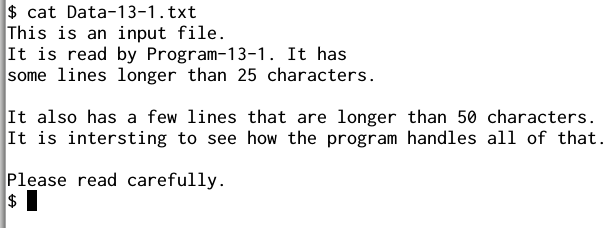
\includegraphics[scale=0.6]{Input-13-1.png}
\caption{Character Input}
\label{input-13-1}
\end{center}
\end{figure}

\lstinputlisting{Program-13-1.c} 

\begin{figure}[ht]
\begin{center}
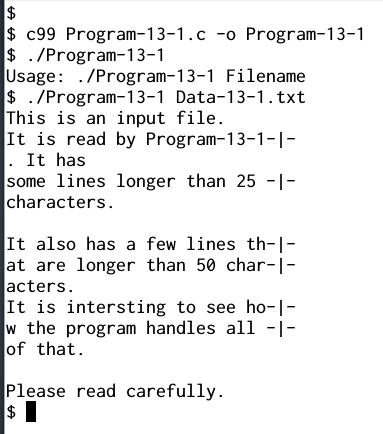
\includegraphics[scale=0.6]{Output-13-1.png}
\caption{Character I/O}
\label{output-13-1}
\end{center}
\end{figure}

Now let us write another program that read the same input file, removes all newlines (`$\backslash$n'), adds a space after the period, and writes it to an output file one character at a time.

\lstinputlisting{Program-13-2.c}

Note how the \lstinline!continue! statement is used in this program.

When we run the program this is what we see:
\begin{figure}[ht]
\begin{center}
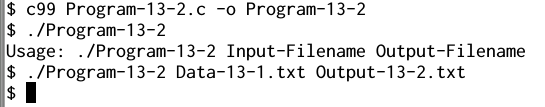
\includegraphics[scale=0.6]{Output-13-2.png}
\caption{Character I/O}
\label{output-13-2}
\end{center}
\end{figure}

Here is how the file looks when opened in vim:
\begin{figure}[ht]

\begin{center}
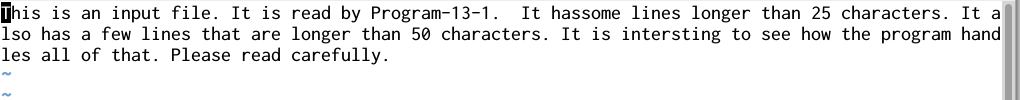
\includegraphics[scale=0.4]{Output-Edit-13-2.png}
\caption{Character I/O}
\label{output-edit-13-2}
\end{center}
\end{figure}
 
\subsubsection*{String I/O}
Here we will read a file line by line, using \texttt{fgets()} and write the output also line by line using \texttt{fputs()}. We will output each line with its line number.

Note the use of the function \texttt{sprintf()} in this code.

\lstinputlisting{Program-13-3.c}

\begin{figure}[ht]
\begin{center}
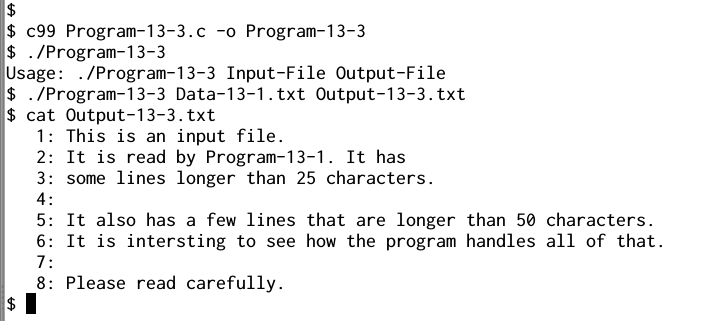
\includegraphics[scale=0.4]{Output-13-3.png}
\caption{String I/O}
\label{output-13-3}
\end{center}
\end{figure}

We can rewrite this program to use \texttt{fprintf()}. In this case it also becomes simpler.

\lstinputlisting{Program-13-3A.c}

We use \texttt{diff} utility to check that two files are identical.
\begin{figure}[ht]
\begin{center}
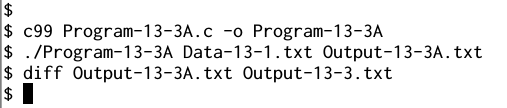
\includegraphics[scale=0.6]{Output-13-3A.png}
\caption{String I/O}
\label{output-13-3A}
\end{center}
\end{figure}
\end{document}